% Standalone TikZ diagram. Copy to figures/tikz/<stem>.tex; built by `./ra figs` into figures/<stem>.pdf.
\documentclass[tikz,border=2pt]{standalone}
\usetikzlibrary{arrows.meta,positioning}
\begin{document}
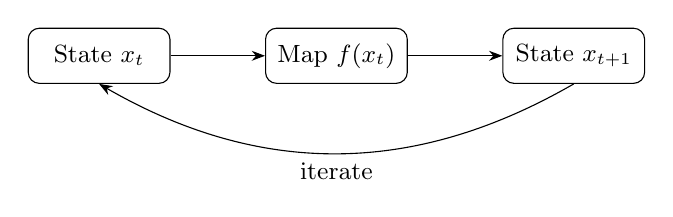
\begin{tikzpicture}[>=Stealth, node distance=12mm, every node/.style={font=\small},
  box/.style={draw, rounded corners, minimum width=18mm, minimum height=7mm}]
  \node[box] (a) {State $x_t$};
  \node[box, right=of a] (b) {Map $f(x_t)$};
  \node[box, right=of b] (c) {State $x_{t+1}$};
  \draw[->] (a) -- (b);
  \draw[->] (b) -- (c);
  \draw[->] (c.south) to[bend left=30] node[below] {iterate} (a.south);
\end{tikzpicture}
\end{document}
